\documentclass[11pt,a4paper]{article}
\usepackage[T1]{fontenc}
\usepackage[utf8]{inputenc}
\usepackage{lmodern}
\usepackage[margin=24mm,headheight=15pt]{geometry}
\usepackage{amsmath,amssymb,mathtools,bm}
\usepackage{graphicx,booktabs,array}
\usepackage{microtype}
\usepackage[numbers,sort&compress]{natbib}
\usepackage{xcolor}
\usepackage{fancyhdr}
\usepackage{hyperref}
\hypersetup{colorlinks=true,linkcolor=blue!45!black,citecolor=blue!45!black,
 urlcolor=blue!45!black,pdftitle={Angular Selection Rules and Time-Delay Relations for Berger--Hopf Lensing in a Closed Cosmology},
 pdfauthor={Norman P. Carberry}}
\pagestyle{fancy}
\fancyhf{}
\fancyhead[L]{\small Berger--Hopf angular light transfer}
\fancyhead[R]{\small Author review draft}
\fancyfoot[C]{\thepage}
\setlength{\parskip}{0.35em}
\setlength{\parindent}{1.1em}
\setlength{\emergencystretch}{2em}
\renewcommand{\topfraction}{0.9}
\renewcommand{\textfraction}{0.08}
\renewcommand{\floatpagefraction}{0.8}
\title{\textbf{Angular Selection Rules and Time-Delay Relations for
Berger--Hopf Lensing in a Closed Cosmology}}
\author{Norman P. Carberry\\[3pt]
\small Independent Researcher, Oconomowoc, Wisconsin, USA\\
\small \href{mailto:carberry8878130@hotmail.com}{carberry8878130@hotmail.com}\\
\small ORCID: \href{https://orcid.org/0009-0000-6650-3485}{0009-0000-6650-3485}}
\date{}

\begin{document}
\maketitle
\begin{center}
\small Research article draft for \emph{Galaxies}: Strong Gravitational Lens Modeling
\end{center}
\begin{abstract}
We calculate angular light transfer and linked strong-lensing time delays
in a conditional effective realization of the Berger--Hopf framework.
The calculation retains the full nine-dimensional scalar $n=2$ harmonic
space of a closed spatial geometry and six physical initial coordinates
for each harmonic. Its observer-centered angular decomposition contains
one monopole, three dipoles and five quadrupoles. Only the quadrupoles
source first-order smooth tracefree beam deformation. We combine their
normalized spatial Hessians with an action-derived temporal propagator
to obtain the observer--lens, observer--source and lens--source response
matrices. A specified quadrupole has a nodal central ray with vanishing
first-order frequency and trace responses but nonzero tidal deformation.
For a fixed physical singular isothermal lens and source displacement,
the resulting relative-delay correction is proportional to
$\cos(2\varphi)$ and to a difference of two propagation kernels.
An illustrative normalized matter-density coefficient of $10^{-3}$ gives
a $-0.353216$ s shift at $(z_l,z_s)=(0.3,1)$ along one screen axis,
the opposite shift after a $90^\circ$ source rotation, and a first-order
null at $45^\circ$. Independent angular-ray and stationary-image
calculations check the result. We give an exact effective-potential
representation and a restricted source-redshift consistency contrast.
These are reproducible conditional predictions; neither an observed
amplitude nor a unique microscopic state is selected.
\end{abstract}
\noindent\textbf{Keywords:} strong gravitational lensing; time delays;
closed cosmology; scalar harmonics; Jacobi maps; Berger--Hopf framework

\section{Introduction}

Strong-lensing calculations connect a physical preparation of geometry and
matter to image positions, beam distortions and arrival times. In the
Berger--Hopf framework used here, the lensing encounter is interpreted as
light traversing an envelope together with its environmental state. A
useful calculation must therefore specify one common smooth environmental
state for the incoming and outgoing propagation, together with the physical
local encounter. Here the local lens is separately prescribed and held
fixed. The calculation must determine which optical quantities this joint
preparation fixes.
This paper develops such a conditional forward calculation for an angular
sector that supports nonzero tidal light transfer.

The retained effective realization, denoted R1 in the accompanying source
archive, is a cubic scalar--tensor action coupled to dust and radiation
on a closed homogeneous background
\cite{Carberry2026EnvironmentalSource,Carberry2026TransportSource}.
We use its six-dimensional linear initial-value problem to supply the
temporal metric responses. We then extend the optical calculation to the
entire scalar $n=2$ spatial eigenspace. This gives a precise question:
\emph{which angular beam distortions and relative arrival-time changes
must accompany one specified preparation of this state?}
The answer is a family of normalized response coefficients and, for one
explicit preparation, a nonzero timing law.

The mathematical ingredients have established precedents. Harmonics on
the three-sphere provide the spatial mode decomposition
\cite{Lindblom2017Harmonics}; scalar shear is a spin-two optical response
\cite{Bernardeau2010FullSky}; and general distance-matrix lens theory
supplies the physical arrival-time function
\cite{Fleury2021Arbitrary,Schneider2019Multiplane}. The contribution here
is their explicit composition with the declared six-state dynamics, the
calculated redshift-dependent coefficients, and the linked angular
shear--delay prediction. The monopole/dipole selection rule and the
generic matrix Fermat construction are used as established geometry,
with derivations included to fix normalization and signs.

The interpretation also requires care. A calculated envelope response can
have an ordinary effective lens-potential representation. Such a
correspondence is compatible with the BHSM interpretation of the same
surface contributions. We construct that representation explicitly;
we do not require a discrepancy from conventional lensing for the forward
calculation to be meaningful. Conversely, a nonzero conditional response
does not by itself identify the physical state from observed images.
Mass-sheet and source-position freedoms remain relevant
\cite{Schneider2019Multiplane,SchneiderSluse2014SPT}.

This is a separate theoretical and computational study. Its inputs are
the stated effective action, frozen homogeneous background, normalized
initial coordinates and prescribed thin-lens encounter. No quasar
photometry, telescope pixels, astrometric fit, detector calibration or
observationally fitted state amplitude enters the calculation.

\section{Physical preparation and approximation}
\label{sec:preparation}

\subsection{Effective dynamics and state coordinates}

With signature $(-,+,+,+)$, the effective action is
\begin{equation}
 S=\int d^4x\sqrt{-g}\left[
 \frac{M_{\rm Pl}^2}{2}\mathcal R
 -\frac12(\nabla T)^2
 +\frac{(\nabla T)^2\Box T}{\Lambda^3}
 -V(T)+\mathcal L_m+\mathcal L_r\right],
 \qquad V(T)=V_0-\mu^3T.
 \label{eq:effective-action}
\end{equation}
The cubic interaction belongs to the established kinetic-gravity-braiding
and generalized scalar--tensor action class
\cite{Deffayet2010Braiding,Kobayashi2011Generalized}.
Its form is not claimed as a new interaction in this work.
Here $T$ is the scalar field, $\mathcal R$ the spacetime Ricci scalar,
and the two matter sectors are pressureless dust and radiation.
The symbol $T$ used later for the time-delay \emph{matrix} is always
distinguished by its matrix equation and context. The numerical provider
uses $M_{\rm Pl}=H_0=c=1$, with rescaled cubic parameter
$\lambda=\Lambda^3/(M_{\rm Pl}H_0^2)$ and slope
$q_T=\mu^3/(M_{\rm Pl}H_0^2)$. Its parameters are
\begin{equation}
 \Omega_{m0}=0.31,\quad\Omega_{r0}=9\times10^{-5},\quad
 \Omega_{k0}=-0.018,\quad K=0.018,\quad
 \lambda=1,\quad q_T=3.
 \label{eq:background-values}
\end{equation}
The frozen background uses $V_0=2.3986073449708067$ in
$M_{\rm Pl}^2H_0^2$ units and the archived
homogeneous initial conditions; it is reused without tuning to any lens.
Appendix~\ref{app:action-provider} describes those conditions and the
quadratic-action reduction.

Each real normalized $n=2$ harmonic carries the physical initial vector
at $z_i=2.1$,
\begin{equation}
 y=\left(\zeta,\Pi_{2,\mathrm{ref}},
 \delta_m^{\mathrm{ADM}},\delta_r^{\mathrm{ADM}},
 v_m^{\mathrm{ADM}},v_r^{\mathrm{ADM}}\right)_i^T.
 \label{eq:physical-anchor}
\end{equation}
The labels specify the gauge and normalization of the input coordinates;
they are not six independently fitted properties of a particular lens.
The reference momentum $\Pi_{2,\mathrm{ref}}$ is converted to the full
canonical state together with the other five inputs. It is not identified
with the canonical momentum of the coupled scalar--matter system.
Rotational symmetry of the homogeneous background makes the same
temporal propagator applicable to every member of the $n=2$ eigenspace.
It does not select their angular coefficients or a preferred axis.

This effective action is a declared conditional realization within the
BHSM research program. The paper does not derive it as a unique
microscopic closure or compute a unique normalized local envelope state.
The physical content of the results is consequently of the form:
\emph{given this effective action and this initial preparation, these
optical responses follow}. The explicitly retained dust and radiation
coordinates permit environmental perturbations to participate in that
prediction.

\subsection{Optical experiment}

Lengths in the field and propagation calculation are measured in $c/H_0$.
The normalized harmonics and their coefficients use that same coordinate
unit; numerical comparisons of different state coordinates therefore
refer to the declared basis. A value $H_0=67.4\,
\mathrm{km\,s^{-1}\,Mpc^{-1}}$ is used only to turn the illustrative
distances, fixed physical source displacement and delays into conventional
units. All lens/source redshifts in the examples lie below the initial
surface at $z_i=2.1$.

We retain terms linear in the smooth scalar perturbations and quadratic
in paraxial transverse separations. A local weak-field thin lens supplies
the strong-lensing encounter. ``Strong'' describes the multiple imaging;
it does not require a strong local metric perturbation. The local
potential is held fixed when the smooth environmental preparation is
varied. In the numerical example it is a singular isothermal sphere
(SIS), prescribed as an effective physical lens. Its microscopic source
and a fully matched nonlinear body solution are not derived here.

The observable delay is measured by the observer's clock at fixed
measured lens and source redshifts. The comparison also fixes the
transverse \emph{physical} source displacement and the physical lens
strength. This choice is part of the experiment: fixing the angular
source position instead changes the derivative. The smooth background
Jacobi maps describe one common narrow beam; spatial variation across a
finite field beyond the retained paraxial order is outside the calculation.
All maps use one parallel-transported screen and nonconjugate vertex
pairs. The measured redshifts specify the reference vertices; no
image-specific endpoint retuning is performed. The SIS is a local
encounter model, rather than a global finite-mass galaxy solution, and
its structural reaction to a changing environment is outside this
fixed-body experiment.

\section{Normalized angular sectors and optical selection}
\label{sec:angular-selection}

Let $R=K^{-1/2}$, $u=\chi/R$, and
$S_K(\chi)=R\sin u$.  The spatial metric is
$\gamma=d\chi^2+S_K^2d\Omega^2$.
Write the unit-sphere embedding coordinates as
$X^0=\cos u$, $X^i=\sin u\,n^i$.
For a real symmetric tracefree $4\times4$ matrix $A$, define
\begin{equation}
 Q_A=\mathcal N X^I A_{IJ}X^J,
 \qquad \mathcal N=\sqrt{\frac{6}{\pi^2R^3}}.
 \label{eq:normalized-harmonic}
\end{equation}
The ambient polynomial is homogeneous harmonic of degree two; hence
$D^2Q_A=-8KQ_A$.  The fourth moment
$\langle X_I X_J X_K X_L\rangle=
(\delta_{IJ}\delta_{KL}+\delta_{IK}\delta_{JL}
+\delta_{IL}\delta_{JK})/24$ gives
\begin{equation}
 \int_{S^3(R)}Q_AQ_B\,dV_\gamma=\operatorname{Tr}(AB).
 \label{eq:harmonic-normalization}
\end{equation}
A Frobenius-orthonormal matrix basis therefore supplies all nine normalized
$n=2$ harmonics.  Decomposing
$A_{ij}=C_{ij}-A_{00}\delta_{ij}/3$, $\operatorname{Tr}C=0$, yields
\begin{align}
 Q_A/\mathcal N={}&A_{00}(\cos^2u-\tfrac13\sin^2u)
 +2A_{0i}\sin u\cos u\,n^i\nonumber\\
 &+\sin^2u\,n^iC_{ij}n^j.
 \label{eq:angular-decomposition}
\end{align}
These are the $1+3+5$ dimensions of the observer-centered angular sectors
$\ell=0,1,2$.  The spatial harmonic index $n$ on $S^3$ and the angular
index $\ell$ on the observer's sky are distinct.

For a screen $E$ satisfying $E^TE=I_2$, $E^Tn=0$, the tracefree spatial
Hessian of $f(\chi)Y_{\ell m}$ is
\begin{equation}
 (D_{\hat A}D_{\hat B}[fY])_{\mathrm{TF}}
 =\frac{f}{S_K^2}
 \left(\nabla_A\nabla_BY-\frac12s_{AB}\Delta_\Omega Y\right).
 \label{eq:screen-hessian}
\end{equation}
The radial connection contribution is proportional to $I_2$.
For $\ell=1$, $\nabla_A\nabla_BY=-s_{AB}Y$ and
$\Delta_\Omega Y=-2Y$, so the bracket vanishes.
The $\ell=0$ bracket also vanishes.  Thus the four monopole/dipole
spatial modes do not source first-order smooth cosmological shear on
observer-centered radial background rays.  This statement does not
remove their trace, redshift or timing responses, and does not remove
shear produced by the galaxy encounter.

For a normalized quadrupole $Q_C=\mathcal N\sin^2u\,n^TCn$ with
$\operatorname{Tr}(C^2)=1$, let
\begin{equation}
 H_C(n)=2E^TCE+(n^TCn)I_2.
 \label{eq:quadrupole-screen-shape}
\end{equation}
This matrix is symmetric and tracefree.  The exact cancellation of the
radial factor gives
\begin{equation}
 (D_{\hat A}D_{\hat B}Q_C)_{\mathrm{TF}}
 =\mathcal N K H_C(n).
 \label{eq:quadrupole-radial-cancellation}
\end{equation}

\section{State-derived tracefree propagation}
\label{sec:tracefree-transfer}

In the convention
$ds^2=a^2[-(1+2\Phi)d\eta^2+(1-2\Psi)\gamma_{ij}dx^idx^j]$,
write the current six temporal metric responses as
$\phi_j(\eta)$ and $\psi_j(\eta)$, and let
$w_j=\phi_j+\psi_j$.
The initial coordinates are
$(\zeta,\Pi_{2,\mathrm{ref}},\delta_m^{\rm ADM},\delta_r^{\rm ADM},
v_m^{\rm ADM},v_r^{\rm ADM})$ for each normalized spatial harmonic.
No equality between the two metric potentials is imposed.

The background physical angle-to-separation map between vertices $a,b$ is
$d_{ab}=a_bS_K(\chi_b-\chi_a)$.
The physical initialization $D'_a=\omega_aI_2$, with one
observer-normalized affine parameter, becomes a unit conformal derivative
at $\chi_a$.  Linearizing the Sachs equation gives
\begin{equation}
 (\partial_\chi^2+K)\delta\widetilde D_{ab}^{\rm TF}
 =-S_K(\chi-\chi_a)
 [D_\perp D_\perp(\Phi+\Psi)]_{\rm TF}.
 \label{eq:linearized-sachs-tf}
\end{equation}
Define shear by $\delta D_{ab}^{\rm TF}=-d_{ab}\Gamma_{ab}$.
For an orthonormal STF three-matrix basis $C_A$, $A=1,\ldots,5$,
the result is
\begin{equation}
 \Gamma_{ab}(n)=\sum_{j=1}^{6}\sum_{A=1}^{5}
 g_{ab,j}y_{jA}H_{C_A}(n),
 \label{eq:shear-response}
\end{equation}
\begin{equation}
 g_{ab,j}=\frac{\mathcal NK}{S_K(\chi_b-\chi_a)}
 \int_{\chi_a}^{\chi_b}S_K(\chi_b-\chi)S_K(\chi-\chi_a)
 w_j(\eta_o-\chi)\,d\chi.
 \label{eq:shear-kernel}
\end{equation}
The three maps $ol$, $os$, and $ls$ are independently initialized.
The final scale $a_b$ cancels from this fractional shear, and no additional
redshift multiplier belongs in the kernel.

At fixed measured redshift, endpoint motion and moving-vertex terms
multiply the background identity at first order.  Corrections to a
first-order shear integral from those shifts are second order.  Local
aberration is conformal on an infinitesimal celestial sphere and supplies
no first-order spin-two term.  These facts establish the tracefree result;
they do not replace the frequency, radial-event and local-scale terms
required for a generic trace response.

The full retained state has 54 coefficients, of which at most 30 enter
this smooth-shear response.  For redshift/vertex labels $r$,
the five angular coefficients satisfy $S_{rA}=G_{rj}y_{jA}$,
$G_{rj}=g_{r,j}$.  A left-null vector of the actual kernel design
therefore supplies a shared-state relation.  Its observational relevance
depends on conditioning, units and the specified lens/source nuisance model.
If all six state components share a single spatial quadrupole $C$,
then $\Gamma_{ab}=(g_{ab}\cdot y)H_C$, and
\begin{equation}
 \gamma_{1,ab}\gamma_{2,cd}-\gamma_{2,ab}\gamma_{1,cd}=0.
 \label{eq:common-profile-alignment}
\end{equation}
This profile restriction is not automatic for a generic six-by-five
quadrupole preparation, and the deterministic identity is not a
stochastic covariance prediction.

\section{A complete conditional timing response on a nodal ray}
\label{sec:nodal-timing}

For a weak thin local potential $\widehat\psi$, use the standard
distance-matrix arrival-time function
\begin{align}
 \beta&=D_{os}^{-1}X_s,
 &T&=(1+z_l)D_{ol}^TD_{ls}^{-1}D_{os},\nonumber\\
 ct(\theta)&=\tfrac12(\theta-\beta)^TT(\theta-\beta)
 -(1+z_l)\widehat\psi(D_{ol}\theta)+f(\beta).
 \label{eq:matrix-fermat}
\end{align}
This optical construction and its clock normalization are established
distance-matrix lens theory \cite{Fleury2021Arbitrary,Schneider2019Multiplane}.
Put $D_{ab}=d_{ab}(I_2+E_{ab})$ and
$T_0=(1+z_l)d_{ol}d_{os}/d_{ls}$.
At first order $\delta T/T_0=E_{ol}+E_{os}-E_{ls}$.
For a stationary image, fixed measured redshifts, fixed transverse
physical source $X_s$, and fixed local physical potential, the source
variation is $\delta\beta=-E_{os}\beta$.
Using the background lens equation and writing $v_i=\theta_i-\beta$,
\begin{equation}
 \frac{c\delta t_i-\delta f}{T_0}
 =\tfrac12v_i^T(E_{os}-E_{ol}-E_{ls})v_i
 +v_i^T(E_{os}-E_{ol})\beta.
 \label{eq:stationary-delay-response}
\end{equation}
The expression includes the varying impact in the local potential.
Image-position derivatives drop out by stationarity; the common $f$
cancels in relative delays.

Choose $C_\star=\operatorname{diag}(1,-1,0)/\sqrt2$, the central ray
$n=e_z$, and screen $(e_x,e_y)$.
Here $Q$ and its full first gradient vanish on the ray, the transverse
Hessian has zero trace, and
$H_{C_\star}=\sqrt2\operatorname{diag}(1,-1)$.
The first-order frequency, radial-event, velocity, local-scale and Jacobi
trace responses therefore vanish.  The first-order physical maps are
fully specified by $E_{ab}=-\Gamma_{ab}$ for this preparation.
These vanishing terms refer to the fiducial nodal ray. Actual images
have small finite angular offsets; their leading tidal separation is
included by the distance matrices. Higher finite-angle corrections
are not bounded by this first-order paraxial calculation.

Take a local SIS, $\widehat\psi(x)=b|x|$, and a source
$X_s=s e$, $e=(\cos\varphi,\sin\varphi)$, with fixed $b,s>0$.
The background values are $\beta=s/d_{os}$,
$\theta_E=bd_{ls}/d_{os}$, and
$\theta_\pm=(\beta\pm\theta_E)e$.
For $0<\beta<\theta_E$ and fixed noncritical branches,
\begin{equation}
 \Delta t_0=t_- -t_+
 =\frac{2(1+z_l)bs}{c}\frac{d_{ol}}{d_{os}}.
 \label{eq:sis-background-delay}
\end{equation}
Since $v_\pm=\pm\theta_E e$, the quadratic term in
Eq.~\eqref{eq:stationary-delay-response} cancels between images:
\begin{equation}
 \boxed{\frac{\delta\Delta t}{\Delta t_0}
 =e^T(\Gamma_{os}-\Gamma_{ol})e
 =\sqrt2[(g_{os}-g_{ol})\cdot y]\cos(2\varphi).}
 \label{eq:quadrupole-delay-law}
\end{equation}
The $ls$ shear cancels for this fixed-physical-source SIS experiment.
The result predicts the angular sign reversal and null directions for
the declared preparation; it does not select the physical amplitude $y$.
It is not a generic prediction for arbitrary galaxy profiles, fixed
angular sources, finite-amplitude metric completions, or higher-order
light propagation.


\section{Executed conditional predictions}
\label{sec:numerical-results}

\subsection{Six response rows}

The constrained quadratic action is evolved from the six unit
preparations in Eq.~\eqref{eq:physical-anchor}. A time-dependent linear
map gives the two Newtonian metric potentials. The sum $\Phi+\Psi$ is
then integrated separately for the $ol$, $os$ and $ls$ maps. This
procedure preserves one common state through all segments while
initializing each physical angle-to-separation map at its own vertex.
Table~\ref{tab:response} gives the resulting response coefficients at
$(z_l,z_s)=(0.3,1)$.

\begin{table}[tbp]
\centering\small
\begin{tabular}{lrrrr}
\toprule
Anchor & $g_{ol,j}$ & $g_{os,j}$ & $g_{ls,j}$ & $k_j=\sqrt2(g_{os,j}-g_{ol,j})$\\
\midrule
$\zeta$ & $-7.589\times10^{-6}$ & $-5.650\times10^{-5}$ & $-2.236\times10^{-5}$ & $-6.918\times10^{-5}$\\
$\Pi_{2,\mathrm{ref}}$ & $6.054\times10^{-5}$ & $1.160\times10^{-3}$ & $6.427\times10^{-4}$ & $1.554\times10^{-3}$\\
$\delta_m^{\rm ADM}$ & $-3.445\times10^{-5}$ & $-4.073\times10^{-4}$ & $-2.042\times10^{-4}$ & $-5.273\times10^{-4}$\\
$\delta_r^{\rm ADM}$ & $-3.005\times10^{-8}$ & $-3.607\times10^{-7}$ & $-1.818\times10^{-7}$ & $-4.675\times10^{-7}$\\
$v_m^{\rm ADM}$ & $3.009\times10^{-4}$ & $3.659\times10^{-3}$ & $1.853\times10^{-3}$ & $4.749\times10^{-3}$\\
$v_r^{\rm ADM}$ & $3.612\times10^{-7}$ & $4.392\times10^{-6}$ & $2.224\times10^{-6}$ & $5.700\times10^{-6}$\\
\bottomrule
\end{tabular}

\caption{Executed unit-state coefficients at $(z_l,z_s)=(0.3,1)$.
The $g$ rows determine fractional shear through
Eq.~\eqref{eq:shear-response}; $k_j$ determines the nodal SIS fractional
delay at $\varphi=0$. Initial coordinates and $L^2$ spatial normalization
are fixed by Eqs.~\eqref{eq:physical-anchor} and
\eqref{eq:harmonic-normalization}. These columns are response derivatives
in that basis, not independently assigned physical perturbation sizes.}
\label{tab:response}
\end{table}

For example, the observer--source density-coordinate response is
$g_{os,\delta_m}=-4.07274462\times10^{-4}$, while the
observer--lens response is $-3.44476439\times10^{-5}$.
Their difference produces
$k_{\delta_m}=-5.27256743\times10^{-4}$.
The nonzero result comes from the evolved environmental preparation
and its integrated transverse Hessian; no measured delay is used to
choose these coefficients.

\subsection{A finite illustrative preparation}

Choose the nodal quadrupole $C_\star$ of
Section~\ref{sec:nodal-timing} and
\begin{equation}
 y_\star=(0,0,10^{-3},0,0,0)^T.
 \label{eq:illustrative-state}
\end{equation}
The number $10^{-3}$ is the coefficient of the normalized harmonic in
the initial ADM matter-density contrast. It does not mean a spatially
uniform $0.1\%$ density perturbation. In particular, its initial spatial
profile is $\delta_m^{\rm ADM}(\chi,n)=10^{-3}Q_{C_\star}(\chi,n)$.
Other components need not stay zero during the coupled evolution.

Set $\sigma_v=200\,\mathrm{km\,s^{-1}}$,
$b=4\pi(\sigma_v/c)^2$, and $s=0.8$ kpc. At
$(z_l,z_s)=(0.3,1)$ the background distances are
\begin{equation}
 (d_{ol},d_{os},d_{ls})
 =(945.162839,1689.312240,1076.994348)\ \mathrm{Mpc}.
\end{equation}
The background source angle is $0.0976799$ arcsec and the Einstein angle
is $0.7354566$ arcsec. The two unperturbed images on the chosen axis lie
at $+0.8331365$ and $-0.6377768$ arcsec. Their baseline relative delay is
$7.75362145$ days. Equation~\eqref{eq:quadrupole-delay-law} gives
\begin{equation}
 \delta\Delta t=-0.35321609\cos(2\varphi)\ \mathrm{s}
 \quad [(z_l,z_s)=(0.3,1),\ y=y_\star].
 \label{eq:executed-delay}
\end{equation}
The source rotation changes its orientation relative to the prepared
quadrupole while keeping its physical displacement magnitude fixed.
This is a family of controlled physical source configurations, not a
rotation of an observed object with all other data held unchanged.

\begin{table}[tbp]
\centering\small
\begin{tabular}{rrrrrr}
\toprule
$z_l$ & $z_s$ & $\Delta t_0$ (days) & $\delta\Delta t(0^\circ)$ (s) & $\delta\Delta t(45^\circ)$ (s) & $\delta\Delta t(90^\circ)$ (s)\\
\midrule
0.3 & 1 & 7.753621 & -0.353216 & 0 & 0.353216\\
0.3 & 0.6 & 9.268876 & -0.123113 & 0 & 0.123113\\
0.5 & 1.5 & 11.583863 & -1.163398 & 0 & 1.163398\\
0.8 & 2 & 17.264699 & -2.871297 & 0 & 2.871297\\
\bottomrule
\end{tabular}

\caption{Conditional first-order delay predictions for the same
normalized preparation, physical SIS strength and physical source
displacement. The source azimuth is measured in the fixed nodal screen.
The $45^\circ$ values are exact first-order zeros; small nonzero values
from a finite linear-map completion do not constitute second-order
field predictions.}
\label{tab:delays}
\end{table}

\begin{figure}[tbp]
\centering
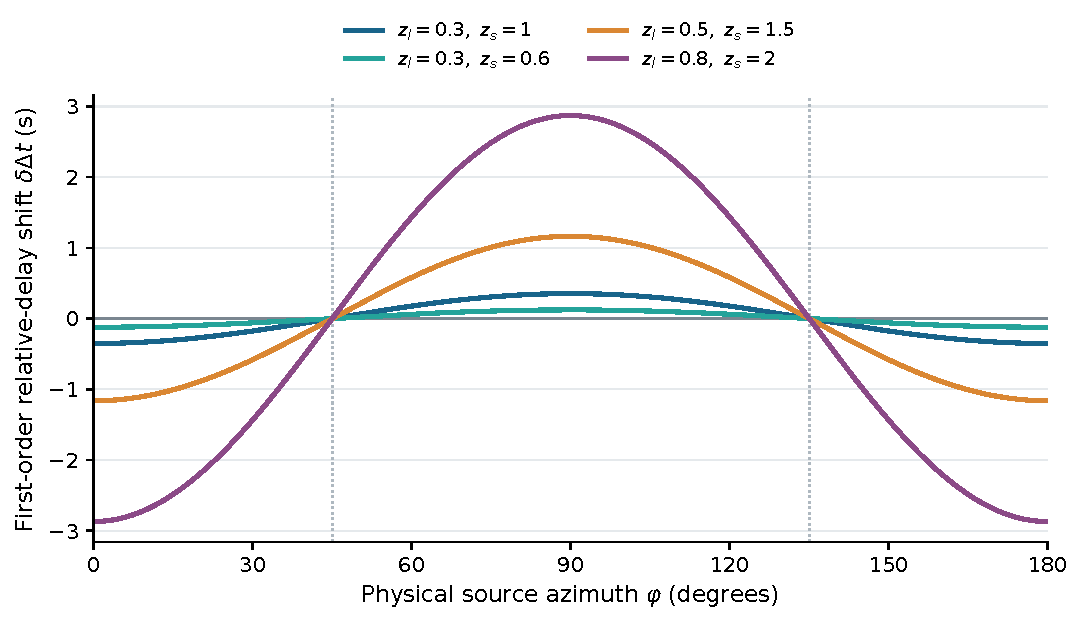
\includegraphics[width=0.98\linewidth]{figures/nodal_delay_angular_response.pdf}
\caption{The calculated angular delay law for the four configurations
in Table~\ref{tab:delays}. Every curve uses the single specified
preparation in Eq.~\eqref{eq:illustrative-state}. The phase, null
directions and sign reversal follow from the common quadrupolar shape;
the amplitudes follow from the six-state propagation and background
distances. The curves are theoretical forward responses.}
\label{fig:angular-delay}
\end{figure}

The larger-redshift examples give larger responses for this chosen state
(Table~\ref{tab:delays}); no universal monotonicity theorem is implied.
Scaling $y_\star$ scales all first-order shifts together. Such a rescaling
does not establish that the resulting amplitude is physically realized or
measurable. At 2001 sampled radial points, exact angular maximization of
the evolved seed gives maximum $2|\Phi|=3.27\times10^{-6}$ through
$z=1$ and $2.04\times10^{-5}$ through $z=2$. The corresponding sampled
first-order matter speeds are $4.89\times10^{-6}c$ and
$1.72\times10^{-5}c$. These values support use of a weak perturbative
illustration on the sampled domain. They are not certified continuous
bounds or a calculation of nonlinear truncation errors.

\subsection{Shared-state relations}

Equation~\eqref{eq:common-profile-alignment} imposes collinearity of the
smooth shear components whenever all six coordinates share one spatial
tensor $C$. An explicit calculation at a generic line of sight and
generic normalized $C$ produces pairwise two-component shear determinants
below $1.01\times10^{-28}$ over the twelve reported propagation
segments. This is a numerical check of the algebraic common-profile
identity. It is not an additional independent constraint on arbitrary
image ellipticities or a statement about noise covariance.

The general preparation contains six independent coefficient sets in
each of five quadrupole directions. For that larger family the useful
restriction is the common temporal response design
$S_{rA}=G_{rj}y_{jA}$. Angular information alone does not select the
six temporal amplitudes. Any proposed inference must also evaluate the
redshift design, its conditioning and the allowed physical nuisance
parameters.

\section{Effective gravitational representation and source-redshift dependence}
\label{sec:representation}

The computed optical response admits a conventional effective-potential
representation. This correspondence is constructive: the geometric and
effective gravitational descriptions encode the same retained light transfer.
The existence of that representation does not identify the physical
preparation from lensing data. Distance-matrix lensing and its associated
degeneracies provide the appropriate comparison
\cite{Fleury2021Arbitrary,Schneider2019Multiplane,SchneiderSluse2014SPT}.

\subsection{Exact correspondence for one source plane}

Use physical angle-to-separation maps in compatible parallel screen frames,
constant across the paraxial beam. Let $T$ be the symmetric time-delay matrix,
$T_0>0$ a scalar reference length, and $M=T/T_0$. The local physical lens
potential $\hat\psi$ and the angular source coordinate
$\boldsymbol\beta=D_{os}^{-1}\boldsymbol X_s$ give
\begin{equation}
 ct(\boldsymbol\theta)
 =\frac12(\boldsymbol\theta-\boldsymbol\beta)^T
 T(\boldsymbol\theta-\boldsymbol\beta)
 -(1+z_l)\hat\psi(D_{ol}\boldsymbol\theta)+f(\boldsymbol\beta).
 \label{eq:representation-original-fermat}
\end{equation}
The arbitrary source-only function $f$ cancels between images of the same
source. Define
\begin{align}
 \boldsymbol\beta_{\rm eff}&=M\boldsymbol\beta,
 \label{eq:representation-effective-source}\\
 \psi_{\rm eff}(\boldsymbol\theta)
 &=\frac{1+z_l}{T_0}\hat\psi(D_{ol}\boldsymbol\theta)
 +\frac12\boldsymbol\theta^T(I-M)\boldsymbol\theta.
 \label{eq:representation-effective-potential}
\end{align}
Expansion of the quadratic terms gives the exact identity
\begin{align}
 \frac{ct(\boldsymbol\theta)}{T_0}
 &=\frac12|\boldsymbol\theta-\boldsymbol\beta_{\rm eff}|^2
   -\psi_{\rm eff}(\boldsymbol\theta)+F_s,\nonumber\\
 F_s&=\frac12\boldsymbol\beta^T(M-M^2)\boldsymbol\beta
       +\frac{f(\boldsymbol\beta)}{T_0}.
 \label{eq:representation-exact-identity}
\end{align}
Since $F_s$ is independent of image position, the stationary images and
relative arrival times are identical in the two representations. The
effective deflection is
\begin{equation}
 \boldsymbol\nabla\psi_{\rm eff}
 =\frac{1+z_l}{T_0}D_{ol}^T
   \hat{\boldsymbol\alpha}(D_{ol}\boldsymbol\theta)
   +(I-M)\boldsymbol\theta.
 \label{eq:representation-effective-deflection}
\end{equation}
This is an application of the established arbitrary-background Fermat
formalism \cite{Fleury2021Arbitrary}; the state-dependent matrices evaluated
here supply its specified cosmological realization.

For the physical SIS potential $\hat\psi(\boldsymbol x)=b|\boldsymbol x|$,
the first term in Eq.~\eqref{eq:representation-effective-potential} is an
elliptical potential when $D_{ol}$ is anisotropic. The quadratic term is a
uniform-convergence and shear contribution. In the nodal quadrupole its
first-order correction is tracefree. Agreement with this effective model
therefore follows from the correspondence and is not separate evidence for
the underlying state. Neither a globally admissible mass distribution nor
agreement with independent dynamical constraints follows from the algebra
alone. Source-position and mass-sheet freedoms must be included when assessing
what an observation can determine \cite{SchneiderSluse2014SPT}.

\subsection{A restricted comparison across two source redshifts}

Consider sources $s$ and $t$ behind the same lens, using the same $D_{ol}$,
physical lens potential, screen frame and small angular patch. For each
source, define background quantities
\begin{align}
 p_s&=\frac{d_{ls}}{d_{os}},&
 T_{0,s}&=(1+z_l)\frac{d_{ol}}{p_s},\nonumber\\
 a_s&=\frac{1+z_l}{T_{0,s}}=\frac{p_s}{d_{ol}},&
 B_s&=I-\frac{T_s}{T_{0,s}}.
 \label{eq:representation-source-scaling}
\end{align}
The equivalent potential has the form
$\psi_{{\rm eff},s}=a_s\hat\psi(D_{ol}\boldsymbol\theta)
+\boldsymbol\theta^TB_s\boldsymbol\theta/2$.
An additional physical quadratic deflector at the main lens,
$\delta\hat\psi(\boldsymbol x)=\boldsymbol x^TA_{\rm lens}\boldsymbol x/2$,
can absorb all these quadratic terms with one fixed symmetric matrix
$A_{\rm lens}$ precisely when
\begin{equation}
 \frac{B_s}{a_s}=D_{ol}^TA_{\rm lens}D_{ol}
 \quad\hbox{is independent of }s.
 \label{eq:representation-physical-quadratic}
\end{equation}
For common nonsingular $D_{ol}$ this is equivalent to source independence
of $B_s/p_s$. To first order about $D_{ol}=d_{ol}I$, it is the familiar
physical-to-reduced scaling $B_s=p_s d_{ol}A_{\rm lens}$.

The tracefree contrast appropriate to the present calculation is
\begin{equation}
 R_{st}=\frac{B_s^{\rm TF}}{p_s}-\frac{B_t^{\rm TF}}{p_t}.
 \label{eq:representation-redshift-contrast}
\end{equation}
With $E_{ab}=-\Gamma_{ab}$ and the common quadrupolar state $y$,
\begin{align}
 B_s^{\rm TF}
   &=[(g_{ol}-g_{ls}+g_{os})\cdot y]H_C+O(|y|^2),\nonumber\\
 R_{st}&=r_{st}H_C+O(|y|^2),\nonumber\\
 r_{st}&=\left[
 \frac{g_{ol}-g_{ls}+g_{os}}{p_s}
 -\frac{g_{ol}-g_{lt}+g_{ot}}{p_t}
 \right]\cdot y.
 \label{eq:representation-state-contrast}
\end{align}
A thin tidal forcing exactly at the main-lens position provides a useful
check: $g_{ol}=g_{ls}=0$ and
$g_{os}\propto S_K(\chi_l)S_K(\chi_s-\chi_l)/S_K(\chi_s)
=S_K(\chi_l)p_s$. Its contrast vanishes, whereas a distributed response
need not obey that scaling.

For the specified nodal tensor
$C_\star=\operatorname{diag}(1,-1,0)/\sqrt2$, the illustrative state with
$y_{\delta_m}=10^{-3}$ and all other initial amplitudes zero gives, at
$z_l=0.3$, $z_s=1$ and $z_t=0.6$,
\begin{equation}
 R_{st}=
 -9.2059866\times10^{-8}
 \begin{pmatrix}1&0\\0&-1\end{pmatrix}
 \quad\hbox{at first order}.
 \label{eq:representation-computed-contrast}
\end{equation}
This dimensionless response cannot be absorbed into the one fixed physical
main-plane quadratic term specified above. It remains compatible with a
distributed conventional gravitational representation of the same light
transfer. The coefficients $B_s$ are model quantities whose inference requires
source, lens and measurement modeling; Eq.~\eqref{eq:representation-computed-contrast}
is not a detected astronomical residual.

In particular, the contrast does not establish general degeneracy breaking.
Nonquadratic lens freedom, source-position transformations, additional lens
planes and uncertain distance factors require their own joint treatment.
Generalized mass-sheet transformations can scale delays for multiple source
planes together \cite{Schneider2019Multiplane}. The result here is narrower:
one shared preparation predicts a definite redshift dependence of its
effective quadratic contribution, and that dependence is constrained when
the physical deflector is required to be shared.


\begin{figure}[tbp]
\centering
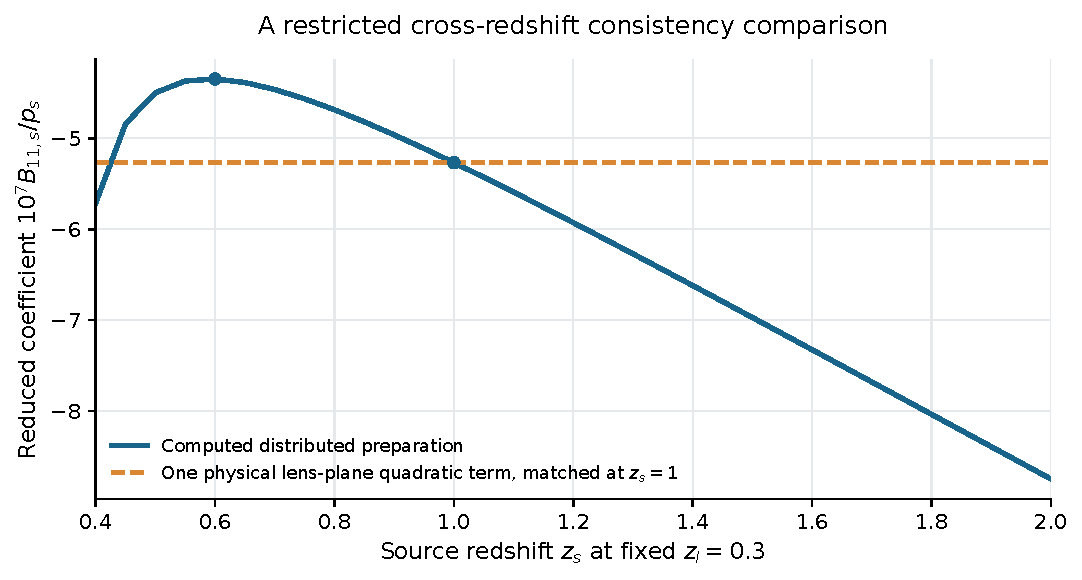
\includegraphics[width=0.98\linewidth]{figures/shared_state_redshift_contrast.pdf}
\caption{The calculated first-order nodal coefficient $B_{11,s}/p_s$
for the same normalized density preparation and $z_l=0.3$, sampled at
33 source redshifts. The dashed comparison is a single fixed physical
quadratic potential at the main lens, matched at $z_s=1$. The contrast
tests that restricted absorption criterion. It is not a direct observable
or an exclusion of distributed gravitational structure, other lens
profiles or generalized mass-sheet freedom.}
\label{fig:redshift-contrast}
\end{figure}

\section{Verification and reproducibility}
\label{sec:verification}

The package separates inherited inputs, new analytic identities,
executed response arrays, lens applications and independent checks.
The inherited source files are exact blobs from a named commit; their
Git identities, SHA-256 hashes and byte lengths are recorded. The
historical manifest is retained for provenance, but only its frozen
background fields enter this calculation. Historical observational
entries in that file are inert.

The main temporal integration uses 801 interpolation points, with a
1601-point refinement and tighter integration tolerances. Each
Green-function shear integral is compared with a separately integrated
forced Jacobi equation. A further check integrates the original angular
Euler momentum equation on the nodal geometry, rather than reusing the
Green kernel. The angle and momentum variables satisfy
\begin{equation}
 \theta'=\frac{L}{S_K^2(\chi)},\qquad
 L'=-w(\eta_o-\chi)\mathcal N\sin^2(\chi/R)\,h\theta,
 \qquad h=\pm\sqrt2,
 \label{eq:independent-angular-ray}
\end{equation}
with the appropriate independently initialized vertex conditions.
Here $w=\sum_j(\phi_j+\psi_j)y_j$ is the temporal Weyl coefficient
for the prepared state, and primes denote $d/d\chi$.
Complex-step and real finite-difference derivatives agree with the
kernel result. The apparent coordinate singularity at the observer is
handled through the regular background initialization described in the
executable audit.

The strong-lensing calculation solves the two noncaustic image branches
and evaluates the full matrix Fermat function. Four-point derivatives
in independent map perturbations reproduce the stationary-image
formula. A separate check reconstructs the SIS baseline directly in
SI units and retains the time-matrix, source-angle and physical-impact
variations before simplification. The effective-potential identity is
checked both in its value, up to a source-only constant, and in its
angular gradient.

\begin{table}[tbp]
\centering\small
\begin{tabular}{p{0.68\linewidth}r}
\toprule
Check & Maximum discrepancy\\
\midrule
$S^3$ harmonic Gram matrix versus $I_9$ (volume quadrature)
 & $3.49\times10^{-14}$\\
Six physical anchors reconstructed from the canonical initial state
 & $2.22\times10^{-16}$\\
Original action constraints, scaled by $\max(1,\|\boldsymbol w\|_\infty)$
 & $1.46\times10^{-11}$\\
Green kernel versus forced Jacobi equation, absolute coefficient
 & $1.45\times10^{-14}$\\
Refined temporal integration, absolute kernel coefficient
 & $1.47\times10^{-13}$\\
Original angular-ray derivative versus kernel, complex-step
 & $2.08\times10^{-15}$\\
Original angular-ray derivative, real half-step comparison
 & $5.70\times10^{-13}$\\
Full image-solve fractional delay derivative versus analytic law
 & $7.12\times10^{-12}$\\
SI baseline reconstruction, relative delay discrepancy
 & $6.24\times10^{-16}$\\
Effective-potential Fermat/gradient identity, scaled
 & $2.01\times10^{-16}$\\
\bottomrule
\end{tabular}
\caption{Executed checks of the declared equations and their numerical
application. The rows use the indicated normalizations; their values
are not interchangeable observational uncertainties or bounds on
omitted physical terms.}
\label{tab:verification}
\end{table}

The finite-map experiment sets $D_{ab}=d_{ab}(I-\Gamma_{ab})$ at a
small finite input and recomputes the images. It checks the derivative
of that map construction. Products generated by this completion are
not a second-order solution of Eq.~\eqref{eq:effective-action}.
In particular, its nonzero residual at the $45^\circ$ first-order null
is not promoted to a new physical prediction. Numerical precision is
kept distinct from the approximation order and physical preparation.

\section{Scientific interpretation and limits}
\label{sec:discussion}

The forward calculation establishes a concrete connection between the
state and two kinds of light response. The spatial harmonic determines
the screen tensor, while the same six-state temporal evolution fixes
the segment-dependent amplitudes. The SIS experiment then reduces a
full stationary arrival-time variation to a difference of two such
amplitudes. The angular orientation of the quadrupole, its timing
amplitude and its shear pattern cannot be assigned independently within this declared
preparation.

The special nodal geometry makes the result particularly transparent.
The fiducial light ray has no first-order scalar frequency or radial
shift, yet the neighboring rays feel a nonzero transverse tidal field.
This permits a complete first-order relative-delay calculation within
the specified paraxial experiment. A generic sightline would require
the trace, endpoint and frequency responses as well. The tracefree
kernel in Eq.~\eqref{eq:shear-kernel} remains useful there, but it cannot
stand in for the missing scalar distance calculation.

There are several distinct levels of physical specification. The
effective action and homogeneous background are fixed inputs. The
initial vector and spatial profile are explicit conditional choices.
The SIS is a prescribed local physical encounter. No observed amplitude,
unique microscopic envelope state, stable nonlinear completion or
population-level distribution of quadrupole orientations is inferred.
Each of these would add physical content beyond the calculations
reported here.

The representation result explains why a successful forward calculation
need not appear as an extra contribution when expressed in familiar
lens variables. Its effective potential already contains the propagated
response. Adding an independent copy of the same surface contribution
would double count it. The restricted redshift contrast gives a way to
state one common-physical-lens condition precisely, while leaving the
broader class of distributed gravitational representations available.

Observational identification is a separate problem. Locally, let
\begin{equation}
 \delta\mathcal O=\mathsf B\,\delta y+
 \mathsf N\,\delta\eta+\epsilon,
 \qquad
 \mathsf B_\perp=(I-P_{W\mathsf N})W\mathsf B,
 \qquad W^TW=\mathsf C^{-1}.
 \label{eq:identifiability}
\end{equation}
Here $\mathsf C$ is the observational covariance, $\eta$ denotes the
allowed lens, source and environmental nuisance parameters, and
$P_{W\mathsf N}$ projects onto their whitened response columns. The rank
and conditioning of $\mathsf B_\perp$ determine which local state
directions survive those freedoms. No such data covariance or fully
specified observational nuisance design is supplied by the present
forward example, so it supplies no detection significance or achievable
parameter error. Generalized mass-sheet transformations can rescale
relative delays together; multiple source redshifts or delay ratios
alone do not guarantee identification \cite{Schneider2019Multiplane}.

A useful next observational design would specify one common preparation
for several source redshifts, a physically constrained main lens and
line-of-sight environment, and independent information on the source
or lens dynamics. The response rows calculated here would then be inputs
to that design. Giving every image or source its own unconstrained
initial state would remove the shared-state relation that motivates
the calculation.

\section{Conclusions}

The full scalar $n=2$ family of the declared closed BHSM/R1 realization
supports an explicit angular optical calculation. Its nine spatial
modes decompose into $1+3+5$ sky sectors. The four monopole/dipole
directions are absent from first-order smooth shear, while the five
quadrupoles have a simple normalized transverse Hessian. Combining
that Hessian with the six physical temporal responses gives the tracefree
parts of the three propagation maps. On the specified nodal ray these
also give the full first-order maps for the retained lens experiment.

For one common nodal quadrupole and a fixed physical SIS/source
preparation, the delay obeys
$\delta\Delta t/\Delta t_0=
\sqrt2[(g_{os}-g_{ol})\cdot y]\cos(2\varphi)$.
The computed example gives a $0.353216$ s amplitude at
$(z_l,z_s)=(0.3,1)$, with a specified sign, $90^\circ$ sign reversal
and $45^\circ$ first-order null. Independent propagation, image solving
and dimensional reconstruction check the result.

An exact effective-potential correspondence preserves image equations
and relative arrival times for one source plane. A calculated
two-redshift contrast tests absorption into one fixed physical quadratic
term at the main lens, without claiming general degeneracy breaking.
The completed contribution is a reproducible family of conditional
BHSM light-transfer and timing predictions, with the state selection
and observational inference left as explicitly separate physical tasks.

\appendix
\section{Frozen effective action and six-state temporal provider}
\label{app:action-provider}

This appendix specifies the conditional R1 realization used for the temporal
response coefficients.  It retains the coupled scalar, dust, and radiation
system of the environmental and transport source calculations
\cite{Carberry2026EnvironmentalSource,Carberry2026TransportSource}.
It does not infer the microscopic BHSM state or its absolute normalization.
The vendored source files and their hashes identify the precise implementation;
only the background entries of the inherited parameter manifest are used.

\subsection{Action, units, and background}

The metric signature is $(-,+,+,+)$ and dots denote cosmic-time derivatives.
In the code units $H_0=M_{\mathrm{Pl}}=c=1$, the effective action, up to its
constant dimensional prefactor, is
\begin{equation}
 S=\int d^4x\sqrt{-g}\left[
 \frac{\mathcal R}{2}+X-V(T)-\frac{2X}{\lambda}\Box T\right]+S_m+S_r,
 \qquad
 X=-\frac12\nabla_\mu T\nabla^\mu T,
 \quad V(T)=V_0-q_TT .
 \label{eq:app-r1-action}
\end{equation}
Thus the cubic term is $+(\nabla T)^2\Box T/\lambda$, with no additional
factor of $1/2$.  In the convention with dimensional cubic scale $\Lambda$,
$G_3=2X/\Lambda^3$ and $\lambda=\Lambda^3/(M_{\mathrm{Pl}}H_0^2)$ after
rescaling $T_{\rm phys}=M_{\mathrm{Pl}}T$ and time by $H_0^{-1}$.
The fluids are minimally coupled, isentropic, irrotational perfect fluids
with $w_m=0$ and $w_r=1/3$; the dust sound speed is exactly zero.

The frozen parameters are
\begin{equation}
 \begin{split}
 (\Omega_{m0},\Omega_{r0},\Omega_{k0},\lambda,q_T)
 &=(0.31,9\times10^{-5},-0.018,1,3),\\
 V_0&=2.3986073449708067 .
 \end{split}
 \label{eq:app-background-parameters}
\end{equation}
Here $K=-\Omega_{k0}=0.018$ is the spatial curvature in $H_0^2/c^2$ units;
$V_0$ is in $M_{\mathrm{Pl}}^2H_0^2$ units.  With $v=\dot T$, the background
implementation uses
\begin{align}
 J&=v+6Hv^2/\lambda, & \dot J+3HJ&=q_T,\nonumber\\
 \rho_T&=\tfrac12v^2+V+6Hv^3/\lambda,
 &3(H^2+K/a^2)&=\rho_m+\rho_r+\rho_T ,
 \label{eq:app-background-equations}
\end{align}
where $\rho_m=3\Omega_{m0}a^{-3}$ and
$\rho_r=3\Omega_{r0}a^{-4}$.  At $z=100$, the inherited background
prescription sets $T=0$ and $J=2q_T/(9H)$, selecting the positive-$v$
solution jointly with the Friedmann constraint.  The stored $V_0$ comes
from the original $H(a=1)=1$ normalization; this calculation neither repeats
that shooting nor retunes it.  Replaying the frozen input gives
$H(a=1)=0.9999999999811999$, a normalization residual of
$-1.88\times10^{-11}$.
The background is integrated in $N=\ln a$ with DOP853, relative tolerance
$2\times10^{-13}$, absolute tolerance $10^{-15}$, and maximum step $0.005$.

\subsection{Finite harmonic action and reduction}

For one real harmonic, $\int Q^2dV_\gamma=1$ and
$\nabla_\gamma^2Q=-8KQ$.  The scalar-field uniform-$T$ ADM convention uses
lapse perturbation $\alpha$, covariant shift
$N_i=\nabla_i(\chi_{\rm sh}Q)$, and spatial curvature perturbation $\zeta$.
All variables below are harmonic coefficients.  Define
\begin{equation}
 \begin{gathered}
 \boldsymbol{x}=(\zeta,D_m,D_r)^T,\qquad
 D_I=\frac{\delta\rho_I}{\rho_I+p_I}+3\zeta,\qquad
 \boldsymbol{u}=(\alpha,\chi_{\rm sh},v_m,v_r)^T,\\
 \kappa=K/a^2,\qquad b_2=8\kappa,\qquad s_2=5\kappa .
 \end{gathered}
 \label{eq:app-action-variables}
\end{equation}
The symbols $v_m,v_r$ here denote ADM fluid velocity potentials, not the
background field velocity $v$.  Put $h_I=\rho_I+p_I$ and
\begin{equation}
 \Theta=H-v^3/\lambda,\qquad
 \Sigma=\tfrac12v^2+12Hv^3/\lambda-3H^2 .
 \label{eq:app-theta-sigma}
\end{equation}
After algebraically eliminating the spatial fluid-current auxiliaries and
performing the declared integration by parts, the implemented polynomial is
\begin{align}
 \frac{L_2}{a^3}={}&-3\dot\zeta^2+s_2\zeta^2+\Sigma\alpha^2
 +2b_2\Theta\alpha\chi_{\rm sh}-2b_2\dot\zeta\chi_{\rm sh}
 \nonumber\\
 &+6\Theta\alpha\dot\zeta+2s_2\alpha\zeta
 -b_2\kappa\chi_{\rm sh}^2+\sum_{I=m,r}h_I\ell_I,\nonumber\\
 \ell_I={}&
 v_I\dot D_I-\frac{b_2}{2}v_I^2+b_2\chi_{\rm sh}v_I
 -\frac{w_I}{2}(D_I-3\zeta)^2-\alpha(D_I-3\zeta).
 \label{eq:app-finite-action}
\end{align}
This equation specifies every finite Hessian entry used by the provider.
Write it as
\begin{equation}
 L_2/a^3=\tfrac12\boldsymbol{u}^TA\boldsymbol{u}
 +\boldsymbol{u}^T(B\dot{\boldsymbol{x}}+D\boldsymbol{x})
 +\tfrac12\dot{\boldsymbol{x}}^TM_0\dot{\boldsymbol{x}}
 +\tfrac12\boldsymbol{x}^TE\boldsymbol{x} .
 \label{eq:app-block-action}
\end{equation}
The auxiliary equations and their Schur reduction give
\begin{align}
 \boldsymbol{u}&=-A^{-1}(B\dot{\boldsymbol{x}}+D\boldsymbol{x}),\nonumber\\
 M&=M_0-B^TA^{-1}B,\qquad
 L=-B^TA^{-1}D,\qquad V_2=E-D^TA^{-1}D .
 \label{eq:app-schur}
\end{align}
The reduced canonical momentum is
$\boldsymbol{p}=a^3(M\dot{\boldsymbol{x}}+L\boldsymbol{x})$.
Consequently the six-dimensional state
$\boldsymbol{w}=(\boldsymbol{x},\boldsymbol{p})^T$ evolves by
\begin{equation}
 \dot{\boldsymbol{x}}=M^{-1}(a^{-3}\boldsymbol{p}-L\boldsymbol{x}),
 \qquad
 \dot{\boldsymbol{p}}=a^3(L^T\dot{\boldsymbol{x}}+V_2\boldsymbol{x}) .
 \label{eq:app-canonical-evolution}
\end{equation}
Dividing these equations by $H$ defines
$d\boldsymbol{w}/dN=F(N)\boldsymbol{w}$ and the full fundamental matrix
$U'=FU$, $U(N_i)=I_6$.  No projection or restart onto an isolated two-state
sector is performed.  The default propagator tolerances are
$(2\times10^{-10},2\times10^{-12})$, with maximum $N$ step $0.01$;
the refinement uses $(2\times10^{-12},2\times10^{-14})$ and step $0.005$.

\subsection{Physical anchor and optical potential rows}

At $z_i=2.1$, $N_i=-\ln3.1$, the six specified coordinates are
\begin{equation}
 \begin{gathered}
 \boldsymbol{y}=(\zeta,\Pi_{2,\rm ref},
 \delta_m^{\rm ADM},\delta_r^{\rm ADM},v_m^{\rm ADM},v_r^{\rm ADM})_i^T,
 \\
 \Pi_{2,\rm ref}=2a_i^3G_{S,2}^{\rm ref}\dot\zeta_i,
 \qquad
 G_{S,2}^{\rm ref}=\frac{5(r+3)}{r+8},\qquad r=\frac{\Sigma}{\Theta^2}.
 \end{gathered}
 \label{eq:app-physical-anchor}
\end{equation}
The reference factor is the inherited gravity--scalar normalization;
$\Pi_{2,\rm ref}$ is not identified with the coupled canonical momentum
$p_\zeta$.  The current action rows implement
$\delta_m^{\rm ADM}=D_m-3\zeta$,
$\delta_r^{\rm ADM}=\tfrac43(D_r-3\zeta)$, and the reconstructed velocity
potentials.  If $\mathcal B_i\boldsymbol{w}_i=\boldsymbol{y}$ denotes these
six rows, the initial canonical state is obtained by solving this full
system, $\boldsymbol{w}_i=\mathcal B_i^{-1}\boldsymbol{y}$.
All six coordinates are retained independently for every spatial harmonic.

The Newtonian metric convention is
$ds^2=-(1+2\Phi)dt^2+a^2(1-2\Psi)\gamma_{ij}dx^idx^j$.
For one harmonic, $\Phi=\phi Q$ and $\Psi=\psi Q$, with reconstructed rows
\begin{equation}
 \begin{gathered}
 \phi=\alpha+\dot\chi_{\rm sh},\qquad
 \psi=-\zeta-H\chi_{\rm sh},\\
 \delta_I^{\rm N}=(1+w_I)(D_I-3\zeta-3H\chi_{\rm sh}),\qquad
 v_I^{\rm N}=v_I^{\rm ADM}-\chi_{\rm sh} .
 \end{gathered}
 \label{eq:app-newtonian-map}
\end{equation}
The derivative of $\chi_{\rm sh}$ includes both the background dependence
of its reconstruction row and the propagated state.  The code evaluates
the former by a complex-step directional derivative.  Multiplication of
these metric rows by $U(N,N_i)\mathcal B_i^{-1}$ gives the six columns
$\phi_j(N),\psi_j(N)$ used by the optical integrals.  Cubic interpolation
uses 801 temporal samples, repeated with 1601 samples in the refinement.
The reported reconstruction, action-constraint, and independent optical
checks establish numerical consistency of this declared finite system.
They do not establish a general stability theorem, select its initial
state, or supply the missing microscopic BHSM preparation.


\section{Reproduction and source provenance}
\label{app:reproduction}

The accompanying package contains the source, executed JSON receipts,
temporal arrays, exact-identity checks, figures and this manuscript.
The root \texttt{README.md} gives a single replay command and the
individual stages. Python 3.12.14, NumPy 2.3.5, SciPy 1.17.0 and
Matplotlib 3.10.8 were used. Reproduction reads no remote data and
requires no telescope archive access.

The inherited action/background/anchor provider is frozen at commit
\href{https://github.com/ncarberry64/Manuscript-Generation/commit/06cf7c1b85d6605bfee0cc0d07fb2af86a66cae9}{\texttt{06cf7c1}} of the
\emph{Manuscript-Generation} repository. The corresponding environmental
derivation is referenced at commit
\href{https://github.com/ncarberry64/Berger-Hopf-Standard-Model/commit/00614fa0d479a2de78460ca061cc5304cdb610cf}{\texttt{00614fa0}} of the
\emph{Berger-Hopf-Standard-Model} repository. The new angular kernels,
nodal timing application, shared-state contrast and manuscript are
packaged separately. SHA-256 manifests allow the inherited inputs and
new release files to be distinguished.

\section*{Author and disclosure statements for review}

\noindent\textbf{Author contribution.} Norman P. Carberry: conceptual
direction and authorship. The author is responsible for review and
approval of the submitted scientific claims.

\noindent\textbf{Computational assistance.} AI-assisted tools were used
to develop code, draft mathematical exposition and perform separate
implementation reviews. Analytic identities, independent numerical
formulations and executable receipts are supplied so that claims can
be checked without relying on those tools' judgments.

\noindent\textbf{Funding and competing interests.} Author confirmation
is required before submission; no funding or conflict declaration is
inferred from independent-researcher status.

\noindent\textbf{Data availability.} All numerical results in this draft
are synthetic forward calculations from the declared inputs. Their
source and receipts are included in the accompanying reproducibility
package. No human-subject or observational target data were analyzed.

\begingroup
\interlinepenalty=10000
\bibliographystyle{unsrtnat}
\bibliography{references}
\endgroup
\end{document}
